\documentclass[]{article}
\makeatletter\if@twocolumn\PassOptionsToPackage{switch}{lineno}\else\fi\makeatother

\usepackage{amsfonts,amssymb,amsbsy,latexsym,amsmath,tabulary,graphicx,xcolor}

%%%%%%%%%%%%%%%%%%%%%%%%%%%%%%%%%%%%%%%%%%%%%%%%%%%%%%%%%%%%%%%%%%%%%%%%%%
% Following additional macros are required to function some 
% functions which are not available in the class used.
%%%%%%%%%%%%%%%%%%%%%%%%%%%%%%%%%%%%%%%%%%%%%%%%%%%%%%%%%%%%%%%%%%%%%%%%%%
\usepackage{url,multirow,morefloats,floatflt,cancel,tfrupee}
\makeatletter


\AtBeginDocument{\@ifpackageloaded{textcomp}{}{\usepackage{textcomp}}}
\makeatother
\usepackage{colortbl}
\usepackage{xcolor}
\usepackage{pifont}
\usepackage[nointegrals]{wasysym}
\urlstyle{rm}
\makeatletter

%%%For Table column width calculation.
\def\mcWidth#1{\csname TY@F#1\endcsname+\tabcolsep}

%%Hacking center and right align for table
\def\cAlignHack{\rightskip\@flushglue\leftskip\@flushglue\parindent\z@\parfillskip\z@skip}
\def\rAlignHack{\rightskip\z@skip\leftskip\@flushglue \parindent\z@\parfillskip\z@skip}


%\if@twocolumn\usepackage{dblfloatfix}\fi
\usepackage{ifxetex}
\ifxetex\else\if@twocolumn\usepackage{dblfloatfix}\fi\fi

\AtBeginDocument{
\expandafter\ifx\csname eqalign\endcsname\relax
\def\eqalign#1{\null\vcenter{\def\\{\cr}\openup\jot\m@th
  \ialign{\strut$\displaystyle{##}$\hfil&$\displaystyle{{}##}$\hfil
      \crcr#1\crcr}}\,}
\fi
}

%For fixing hardfail when unicode letters appear inside table with endfloat
\AtBeginDocument{%
  \@ifpackageloaded{endfloat}%
   {\renewcommand\efloat@iwrite[1]{\immediate\expandafter\protected@write\csname efloat@post#1\endcsname{}}}{\newif\ifefloat@tables}%
}%

\def\BreakURLText#1{\@tfor\brk@tempa:=#1\do{\brk@tempa\hskip0pt}}
\let\lt=<
\let\gt=>
\def\processVert{\ifmmode|\else\textbar\fi}
\let\processvert\processVert

\@ifundefined{subparagraph}{
\def\subparagraph{\@startsection{paragraph}{5}{2\parindent}{0ex plus 0.1ex minus 0.1ex}%
{0ex}{\normalfont\small\itshape}}%
}{}

% These are now gobbled, so won't appear in the PDF.
\newcommand\role[1]{\unskip}
\newcommand\aucollab[1]{\unskip}
  
\@ifundefined{tsGraphicsScaleX}{\gdef\tsGraphicsScaleX{1}}{}
\@ifundefined{tsGraphicsScaleY}{\gdef\tsGraphicsScaleY{.9}}{}
% To automatically resize figures to fit inside the text area
\def\checkGraphicsWidth{\ifdim\Gin@nat@width>\linewidth
	\tsGraphicsScaleX\linewidth\else\Gin@nat@width\fi}

\def\checkGraphicsHeight{\ifdim\Gin@nat@height>.9\textheight
	\tsGraphicsScaleY\textheight\else\Gin@nat@height\fi}

\def\fixFloatSize#1{}%\@ifundefined{processdelayedfloats}{\setbox0=\hbox{\includegraphics{#1}}\ifnum\wd0<\columnwidth\relax\renewenvironment{figure*}{\begin{figure}}{\end{figure}}\fi}{}}
\let\ts@includegraphics\includegraphics

\def\inlinegraphic[#1]#2{{\edef\@tempa{#1}\edef\baseline@shift{\ifx\@tempa\@empty0\else#1\fi}\edef\tempZ{\the\numexpr(\numexpr(\baseline@shift*\f@size/100))}\protect\raisebox{\tempZ pt}{\ts@includegraphics{#2}}}}

%\renewcommand{\includegraphics}[1]{\ts@includegraphics[width=\checkGraphicsWidth]{#1}}
\AtBeginDocument{\def\includegraphics{\@ifnextchar[{\ts@includegraphics}{\ts@includegraphics[width=\checkGraphicsWidth,height=\checkGraphicsHeight,keepaspectratio]}}}

\DeclareMathAlphabet{\mathpzc}{OT1}{pzc}{m}{it}

\def\URL#1#2{\@ifundefined{href}{#2}{\href{#1}{#2}}}

%%For url break
\def\UrlOrds{\do\*\do\-\do\~\do\'\do\"\do\-}%
\g@addto@macro{\UrlBreaks}{\UrlOrds}



\edef\fntEncoding{\f@encoding}
\def\EUoneEnc{EU1}
\makeatother
\def\floatpagefraction{0.8} 
\def\dblfloatpagefraction{0.8}
\def\style#1#2{#2}
\def\xxxguillemotleft{\fontencoding{T1}\selectfont\guillemotleft}
\def\xxxguillemotright{\fontencoding{T1}\selectfont\guillemotright}
%%%%%%%%%%%%%%%%%%%%%%%%%%%%%%%%%%%%%%%%%%%%%%%%%%%%%%%%%%%%%%%%%%%%%%%%%%

\def\companyName{Primerlabs}
\def\companyShortName{Primer Labs}


\usepackage[paperheight=11in,paperwidth=8.5in,top=0.93in,bottom=1.1in,left=6cm,right=2cm]{geometry}%,headsep=0.3in,footskip=0.49in
\usepackage[hidelinks]{hyperref}
\usepackage{fancyhdr}
\usepackage{tikz}
\usepackage{sans}
\usepackage[absolute]{textpos}
\RequirePackage[titles]{tocloft}
%\usepackage{helvet} 
\newcommand{\newsymb}{
\begin{tikzpicture}
\filldraw[fill=black,draw=yellow] circle (6pt);
\end{tikzpicture}
}



\newcount\cnta
\cftsetpnumwidth{0pt}
\renewcommand\cftsecpagefont {\global\cnta}
\renewcommand\cftsecafterpnum {%
	  \makebox[0pt][l]%
     {\kern-\dimexpr\linewidth+2em\relax\makebox[1em][r]{\the\cnta}}%
}

\makeatletter
\renewcommand*{\l@section}[2]{%
  \ifnum \c@tocdepth >\z@
    \if@cfthaschapter
      \vskip \cftbeforesecskip
    \else
      \addpenalty\@secpenalty
      \addvspace{\cftbeforesecskip}
    \fi
    {%
    \setlength{\cftsecindent}{1em}
    \leftskip \cftsecindent\relax
     \rightskip \@tocrmarg
     \parfillskip -\rightskip
     \raggedright
     \parindent \cftsecindent\relax\@afterindenttrue
     \interlinepenalty\@M
     \leavevmode
     \@tempdima \cftsecnumwidth\relax
     \let\@cftbsnum \cftsecpresnum
     \let\@cftasnum \cftsecaftersnum
     \let\@cftasnumb \cftsecaftersnumb
     \advance\leftskip \@tempdima \null\nobreak\hskip -\leftskip
     \makebox[0pt][r]{\bfseries#2\hspace*{.4em}}%
     {\cftsecfont #1}\nobreak\par}%
  \fi}
\def\author#1{\gdef\@author{\hskip-\dimexpr(\tabcolsep)\hskip1pt\parbox{\dimexpr\textwidth-1pt}{\bfseries\raggedright \textit{#1}}}}

\let\@whiteDate\@empty\def\whiteDate#1{\gdef\@whiteDate{{#1}}}
\def\NormalBaseline{\def\baselinestretch{1.1}}
\def\title#1{\gdef\@title{\raggedright\bfseries\def\baselinestretch{1}\selectfont\selectfont#1}}
\renewenvironment{abstract}
{\hspace*{-15pc}\vspace*{-9.3pc}\vbox to -22pt \bgroup\begin{minipage}{1.7in}{\fontsize{8}{10}\selectfont\addtocontents{toc}{\protect\setcounter{tocdepth}{-1}}\tableofcontents\addtocontents{toc}{\protect\setcounter{tocdepth}{2}}}\vspace{1cm}\end{minipage}\egroup\vspace*{-.4pc}\trivlist\item[]\leftskip1pt\hfill\hfill\mbox{\null}\par\noindent\ignorespaces\color{black} }{\par\noindent\endtrivlist}
\newenvironment{copys}[1][\unskip]{%
\par
\noindent 
\footnotesize
\noindent}
{}
\fancypagestyle{plain}{\renewcommand{\headrulewidth}{0pt}\renewcommand{\footrulewidth}{0pt}\fancyhf{}\fancyhead[L]{\hspace*{-12pc}\companyShortName\space \color{gray!90}White Paper v0.1}}



\fancypagestyle{headings}{\renewcommand{\headrulewidth}{0pt}\fancyhf{}\fancyfoot[R]{\companyShortName \space{\color{gray!90}White Paper v0.1}\quad\thepage}}\pagestyle{headings}


\linespread{1.3}\date{}  
\usepackage[noindentafter,explicit]{titlesec}
\setcounter{secnumdepth}{5}
\usepackage{listings}
\usepackage{color}

\definecolor{mygreen}{rgb}{0,0.6,0}
\definecolor{mygray}{rgb}{0.5,0.5,0.5}
\definecolor{mymauve}{rgb}{0.58,0,0.82}


\lstset{ 
  backgroundcolor=\color{white},   % choose the background color; you must add \usepackage{color} or \usepackage{xcolor}; should come as last argument
  basicstyle=\footnotesize,        % the size of the fonts that are used for the code
  breaklines=true,                 % sets automatic line breaking
  captionpos=b,                    % sets the caption-position to bottom
  commentstyle=\color{mygreen},    % comment style
  deletekeywords={...},            % if you want to delete keywords from the given language
  escapeinside={\%*}{*)},          % if you want to add LaTeX within your code
  extendedchars=true,              % lets you use non-ASCII characters; for 8-bits encodings only, does not work with UTF-8
  keepspaces=true,                 % keeps spaces in text, useful for keeping indentation of code (possibly needs columns=flexible)
  keywordstyle=\color{blue},       % keyword style
  morekeywords={*,...},            % if you want to add more keywords to the set
  numbers=none,                    % where to put the line-numbers; possible values are (none, left, right)
  rulecolor=\color{black},         % if not set, the frame-color may be changed on line-breaks within not-black text (e.g. comments (green here))
  showspaces=false,                % show spaces everywhere adding particular underscores; it overrides 'showstringspaces'
  showstringspaces=false,          % underline spaces within strings only
  showtabs=false,                  % show tabs within strings adding particular underscores
  stepnumber=1,                    % the step between two line-numbers. If it's 1, each line will be numbered
  stringstyle=\color{mymauve},     % string literal style
  tabsize=2,	                   % sets default tabsize to 2 spaces
  title=\lstname                   % show the filename of files included with \lstinputlisting; also try caption instead of title
}
\titleformat{\section}[hang]{\NormalBaseline\filright\large\bfseries\boldmath}
{\large\thesection\hspace{-6pt}}
{10pt}
{#1}
[]
\titleformat{\subsection}[hang]{\NormalBaseline\filright\bfseries\boldmath}
{\thesubsection\hspace{-6pt}}
{10pt}
{#1}
[]
\titleformat{\subsubsection}[hang]{\NormalBaseline\filright\bfseries\boldmath}
{\thesubsubsection\hspace{-6pt}}
{10pt}
{#1\addcontentsline{toc}{subsubsection}{#1 }}
[]
\titleformat{\paragraph}[runin]{\NormalBaseline\filright\bfseries\boldmath}
{\theparagraph\hspace{-6pt}}
{10pt}
{#1}
[]
\titleformat{\subparagraph}[runin]{\NormalBaseline\filright}
{\thesubparagraph\hspace{-6pt}}
{10pt}
{#1}
[]

\titlespacing{\section}{0pt}{1.5\baselineskip}{.2\baselineskip}  
\titlespacing{\subsection}{0pt}{1\baselineskip}{.2\baselineskip}  
\titlespacing{\subsubsection}{0pt}{1.5\baselineskip}{.2\baselineskip}  
\titlespacing{\paragraph}{0pt}{.5\baselineskip}{10pt}  
\titlespacing{\subparagraph}{0pt}{.5\baselineskip}{10pt}               

\addtocontents{toc}
{\begingroup\protect\let\protect\ttl@gmk\protect\relax\protect}
\makeatother
\renewcommand{\contentsname}{\hspace*{-1pc}{Table of contents}}


\usepackage[numbers,sort&compress]{natbib}
\bibliographystyle{abbrvnat}


\def\copyRight{}
\makeatletter\fancypagestyle{plainx}{\renewcommand{\headrulewidth}{0pt}\renewcommand{\footrulewidth}{0pt}\fancyhf{}\fancyfoot[R]{\thepage}\fancyfoot[L]{\begin{copys}\copyRight~\\[8pt]\tiny\copyright\space \the\year\space\companyName.\space All rights reserved.~\\\ifx\@whiteDate\@empty\today\else\@whiteDate\fi\end{copys}}}\makeatother
\begin{document}


\def\authorCount{0}
\def\affCount{0}

\def\journalTitle{White Paper- Primerlabs}

\title{An incremental approach for building an intelligent tutoring system using a dialog based agent}
\author{Siddharth Kanungo}


\maketitle 
\def\RunningTitle{{An incremental approach for building an intelligent tutoring system using a dialog based agent}}
\addcontentsline{toc}{section}{Abstract}
\begin{abstract}
  \textbf{Abstract}
  A text-based conversational agent would allow guided learning to be more personalized and adaptive to the needs of learner. Part of the solution involves creating dialog scripts to be used by agents to instruct the learner about a subject and part of the solution involves developing an interface through which the agent interacts with the learner. Such a system enables the learner to enrich their personal knowledge database and aids in retaining their learning through spaced repetitions. Contrary to popular beliefs, the conversational agent can be an effective tool for learning even without possessing the ability to process natural language. We have built a tutoring system using a dialog based agent called Primer and we state the rationale and architecture of such a system in this paper. 
\end{abstract}
    
\section{Introduction}
The traditional methods for guided learning, such as textbooks, recorded lectures, and instructor-led learning, are insufficient in the dissemination of the vast amount of scientific knowledge that is continuously being generated every year. The idea of building a conversational agent stems from the need that access to the collective scientific knowledge should be made easier. Reasons for the inability to access such large amount to knowledge may be attributed to prerequisites debt, inability to scale traditional methods of learning, inadvertent denial of access, high opportunity costs associated with the pursuit of acquiring knowledge, a high perceived barrier to entry and the issue of self-discipline coupled with low attention span of learners. 

Guided learning in the form of a conversational agent will be able to mitigate such issues. Apart from that, we look into different problems for which guided learning can be an effective tool.
\subsection[Bloom's 2 Sigma]{Bloom's 2 Sigma Problem}
In 1984, educational researcher Benjamin Bloom published his findings\cite{doi:10.3102/0013189X013006004} that using mastery learning, one-on-one tutoring led to a two-sigma improvement in student's performance over the students who were instructed using conventional methods.  In the paper, he posed the question: 
\begin{quote}
  Can researchers and teachers devise teaching-learning conditions that will enable the majority of students under group instruction to attain levels of achievement that (at present) can be reached only under good tutoring conditions?
\end{quote}
This question is referred as the \textbf{Bloom's 2 Sigma problem}. Bloom saw his key factor influencing his findings: one-on-one tutoring is “too costly for most societies to bear on a large scale“.  

Also a study regarding the effectiveness of direct instruction \cite{doi:10.3102/0034654317751919} shows that the effects of direct instruction using mastery learning are large. The paper notes that 
\begin{quote}
  Yet,  despite  the  very  large  
body of research supporting its effectiveness, DI has not been widely embraced or 
implemented
\end{quote}

Due to technological advances, the idea of one-on-one tutoring without a human actor is feasible with the aid of a conversational agent. Although, it's effectiveness compared to human actors led tutoring needs to be improved continuously.
 \subsection[Gatto's Critisicm]{Gatto's Critisicm of Schooling}
 John Taylor Gatto in his book Dumbing us down \cite{gatto2017dumbing} notes that the current widespread schooling system inadvertently teaches the following:
 \begin{enumerate}
  \item \textbf{Confusion}: Teaching out of context, fragmentation, facts loosely or not at all connected to life or other pieces of information.
  \item \textbf{Indifference}: It encourages superficial and shallow understanding of a wide spectrum of subjects rather than deep knowledge of one. The classes are structured based on time allotments and the students are not provided enough time to delve deeply into a subject. Gatto notes that when it's time to move to another class, the student must stop caring or learning about $xyz$ subject and now to focus on $abc$.
  \item \textbf{Class position}: Students are restricted in their assigned class. 
  \item \textbf{Emotional \& intellectual dependency, provisional self-esteem}: Stars, grades, prizes, and honors are often awarded based on the ability of the student for doing what they are told. The expert chooses what to study and who has done a good job.
  \item \textbf{Surveillance}: Schools afford no privacy for students. The movements of students in schools are highly restricted.
\end{enumerate}

Gatto states that the goal of the school is compliance, not curiosity. Similar concerns have been raised by Ivan Illich \cite{illich1973deschooling} and Pawan Gupta\cite{gupta2000liberating}. Ivan Illich suggests creation of Learning Webs to connect learners with "masters" and Pawan Gupta advocates that the schooling should be relatable to the local environments.

In order to counter against such schooling, Gatto advocates homeschooling where the learners are in charge of their own learning. Although homeschooling has never been easier at this point in time in history due to technological advances, its widespread adoption is limited. 

Guided-learning in the form of a conversational agent will be an effective tool for parents to home school their children. The conversational agent can be extended to include local context into the learning lesson so that they students can map their understanding about the world from their local environments. 

\subsection{Deep Work}
In his book, Deep Work \cite{newport2016deep}, computer science professor, Dr.Cal Newport defines deep work as
\begin{quote}
  Professional activities performed in a state of distraction-free concentration that pushes your cognitive capabilities to their limit. These efforts create new value, improve your skill, and are hard to replicate.
  \end{quote}

An undertaking of learning a subject by oneself requires the ability to do deep work frequently over a long period of time. Barbara Oakley in her book Mindshift\cite{oakley2017mindshift} notes that
\begin{quote}
  Becoming an expert in something new, whatever the subject, means building small chunks of knowledge using day-by-day practice and repetitions. Gradually, these small chunks can be knit together into mastery.
\end{quote}



Although deemed revolutionary, Massive Online Organized Courses (MOOCs) have failed to entice most of the students to complete the courses which they had signed up for. This signifies that the obstacle towards self-learning subjects is more affiliated with the self-discipline than the availability of learning materials. This also posits that the responsibility of the tutor is not only to equip the students with the information about the subject but also ensuring mitigation of the known issues pertaining to self-discipline among the learner. 

A conversational agent will help in eliminating a lot of friction in the undertaking by providing digestible chunks of new information, helping in retaining information learned and acting as a personal knowledge database \& assistant.

\subsection[Lockhart's Lament]{A Mathematician's Lament}
In his article A Mathematician's Lament\cite{lockhart2009mathematician}, mathematician Paul Lockhart notes the following: 

\begin{quote}
  If I had to design a mechanism for the express purpose of destroying a child's natural curiosity and love of pattern-making, I couldn't possibly do as good a job as is currently being done. I simply wouldn't have the imagination to come up with the kind of senseless, soul-crushing ideas that constitute contemporary mathematics education.
\end{quote}


The pedagogy of mathematics warrants its careful treatment as an art. Mathematical subjects require that the student approach them as a creative pursuit rather than being dependent on rote learning of formulas and pattern matching. This requires that mathematical topics are needed to be experimented with and improved continuously by gauging their effectiveness at elevating the learner's mathematical aptitude. 


The issue of incorrect pedagogy is also prevalent in other fields of studies as well. And experimenting with the curriculum and the way of introducing new information will result in improvements.

Traditional methods of guided learning have less scope for improvement and less space for experimentation. However, the script and features of the conversational agent can be continuously improved based on feedback resulting in more effectiveness.


\subsection[Eliza Effect]{The Eliza Effect}

In 1966, Computer Scientist Joseph Weizenbaum, created a chatbot program called ELIZA. When executing Weizenbaum's DOCTOR script, ELIZA parodied a psychotherapist, largely by rephrasing the \textit{patient's} replies as question. ELIZA's DOCTOR script was found to be surprisingly successful in eliciting emotional responses from users who, in the course of interacting with the program, began to ascribe understanding and motivation to the program's output. Upon observation, researchers discovered users unconsciously assuming ELIZA's questions implied interest and emotional involvement in the topics discussed, even when they consciously knew that ELIZA did not simulate emotion.

In his book \textit{Fluid concepts and creative analogies}\cite{hofstadter1995fluid}, Douglas Hofstadter refers to this phenomenon as the ELIZA Effect. He defines it as 
\begin{quote}
The susceptibility of people to read far more understanding than is warranted into strings of symbols—especially words—strung together by computers.
\end{quote}


A trivial example of the specific form of the Eliza effect, given by Douglas Hofstadter, involves an automated teller machine which displays the words "THANK YOU" at the end of a transaction. A casual observer might think that the machine is actually expressing gratitude; however, the machine is only printing a preprogrammed string of symbols.

We developed a conversational agent called Primer and in this paper we outline the conceptual framework with the underlying rationale, principles and architecture of the system. This paper challenges the notion that an effective conversational agent will require proficient ability to process natural language. We propose that an effective platform with the agent having no ability to understand natural language can be built by taking advantage of the ELIZA Effect and incrementally improving its ability to understand basic user intent. The goal of building such a system is to provide all those who want to learn with access to an tutor for teaching them at any time in their lives.  

\section{Conceptual Framework}
\subsection[Objectives]{Objectives}

We define the basic objectives of our intelligent tutoring system as follows:
\begin{itemize}
  
  \item the system should be able to instruct a learner regarding a subject in a dialog based format
  \item the system should be able to provide enough learning aids to the learner to deepen the understanding of the subject
  \item the system should be able to assist the learner in revising subject for maximum retention
\end{itemize} 


In order to understand the conceptual framework for building such a tutoring system, we will begin by basing our system on a simplified model of a classroom instructor. We will assume that the way this particular instructor instructs is by following a pre-defined format. We also assume that this particular instructor does not possess any art of storytelling to captivate the students. This particular assumption helps us to base our model such that the lectures consists only of pure information directly associated with the lectures and not any trivial buffer to keep students engaged. We call this system, the unimaginative instructor. We will also assume that the system is teaching is only one student. 

\subsection[Instructor Model]{The blueprint of an unimaginative instructor} 

In order to teach a student a particular course, the unimaginative instructor prepares a curriculum or customizes a widely used one. A curriculum dictates the relative ordering of the course topics for better understanding. The instructor divides the course into sections according to the curriculum  and distributes them over a number of lectures.

The standard template used by the Unimaginative Instructor can be as follows:
\begin{enumerate}
  \item States the topic
  \item Provides historical background and importance of the topic
  \item Shows applications of the topics of the topic
  \item Explain basic concepts and how it fits together with the rest of the course topics  
  \item Shows the derivation of equations and formulaes, if any.
  \item Demonstrates the usage of such equations
  \item Moves to step 1 for the next topic
  \end{enumerate}

The Unimaginative Instructor does the job of conveying of ideas necessary for learning the course pretty well. However, the course comprehension of the student for the course may be low as the student may find the lecture dull and hard to pay attention to.

We can improve students comprehension by introducing interactivity to the instructor. 

\subsection[Conversational Tutor]{Conversational Tutor}


In order to add interactivity, we will convert the lectures from the unimaginative instructor into text format. The lectures would be classified into the following:

\begin{itemize}
  \item \textbf{Information}: A formal presentation of main ideas pertaining to the topic 
  \item \textbf{Interaction}: An interaction is a question or prompt posed to the learner by the system which requires learner input. An interaction consists of:
  
  \begin{enumerate}
    \item \textbf{Conversation}: A short informal and often personalized discussion regarding the topic. In Conversation, the learner could interact with the user using predefined replies or an input text area.
    \item \textbf{Widget}: An interactive teaching aid. Widgets consist of multiple choice questions, reordering, fill in the blanks, match the following, an interactive chessboard, an explorable etc. 
  \end{enumerate}


\end{itemize}

\begin{lstlisting}[frame=single,caption=Learning Atom with Interaction using MCQ Widget with the learner Nell,label=list1]
  %*\textbf{Primer}*) : Nell, what is the answer to the ultimate question of life, the         universe, and everything?
  %*\textbf{Primer}*) : Options are [a]Happiness  [b]42  [c]108  [d]666
  %*\textbf{Nell}*)   : It is [b]42, of course.  
  %*\textbf{Primer}*) : Wrong. It is [a]Happiness and don't let any sci-fi nut tell you        otherwise.
  \end{lstlisting}


Interaction helps in retaining the student's attention and forces the student to attempt to utilize information acquired from the course to submit inputs to the questions posed during in the interaction. 

Each topic is broken down in sets of Interaction and/or Information. Such a set of Interaction and/or Information is named \textbf{Learning Atom} for convenience. 

The main ideas of the topic are communicated using Information, while the Interaction with the learner is done with the help of Conversation and Widgets.  

Listing \ref{list1} shows a Learning Atom with Interaction using MCQ Widget. Listing \ref{list2} shows a Learning Atom with Interaction using \textit{Conversation}.


The goal of each Learning Atom is to increase and test learner's understanding of the subject. In order to do that each Learning Atom is associated with a learning objective based on Revised Bloom’s Taxonomy. 



\begin{figure}
  \makebox[\linewidth]{
    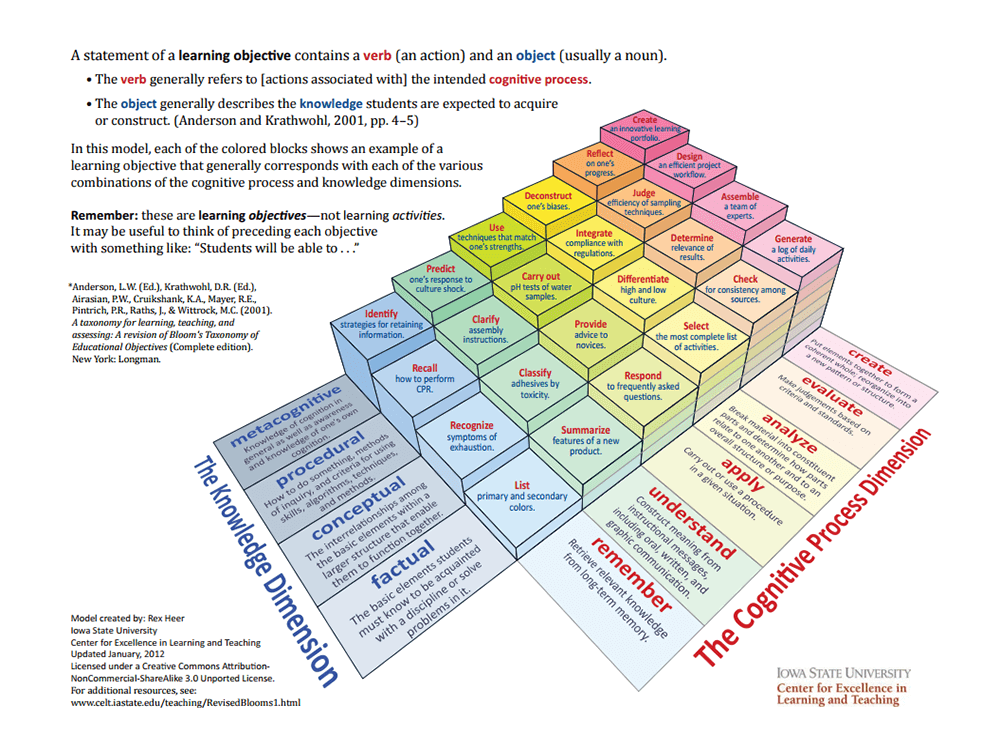
\includegraphics[width=1.2\linewidth]{bloom.png}
    }
    \caption{A 3d representation of Revised Bloom's Taxonomy. Credits to Iowa State University }
    \label{fig1}
\end{figure}

\subsection[Bloom’s Taxonomy]{Revised Bloom’s Taxonomy}
In 1956, Benjamin Bloom headed a group of educational psychologists who developed a classification system for levels of cognitive skills and learning behaviour. The classification system they created is often referred to as Bloom's Taxonomy\cite{bloom1965bloom}.

In 2001, Lorin Anderson and a group of cognitive psychologists, curriculum theorists and instructional researchers, and testing and assessment specialists published a revision of Bloom’s Taxonomy with the title A Taxonomy for Teaching, Learning, and Assessment\cite{anderson2001taxonomy}.

The Revised Bloom's Taxonomy provides a valuable framework to develop performance tasks, creating questions, constructing problems and helps in assessment of the learner's ability. The Taxonomy classifies the learning behaviour into two dimensions:

\begin{enumerate}
  \item Cognitive Process Dimension
  \item Knowledge Dimension
\end{enumerate}

\textbf{Cognitive Process Dimension}
The cognitive process dimension represents a continuum of increasing cognitive complexity from remember to create. Anderson and his group identified 19 specific cognitive processes that further clarify the bounds of the six categories.

\begin{enumerate}
  \item \textbf{Remember}: recognizing (\textit{identifying}), recalling (\textit{retrieving})
  \item \textbf{Understand}:  interpreting \textit{(clarifying, paraphrasing, representing, translating)},
  exemplifying \textit{(illustrating, instantiating)}, 
  classifying \textit{(categorizing, subsuming)},  
  summarizing \textit{(abstracting, generalizing)},  
  inferring \textit{(concluding, extrapolating, interpolating, predicting)},  
  comparing \textit{(contrasting, mapping, matching)},  
  explaining \textit{(constructing models)}
  
  \item \textbf{Apply}: executing \textit{(carrying out)}, implementing \textit{(using)}
  
  \item \textbf{Analyze}:  differentiating \textit{(discriminating, distinguishing, focusing, selecting)},  organizing \textit{(finding, coherence, integrating, outlining, parsing, structuring)}, 
  attributing \textit{(deconstructing)}
  
  \item \textbf{Evaluate}:  checking \textit{(coordinating, detecting, monitoring, testing)},  
  critiquing (\textit{judging})
  
  \item \textbf{Create}: generating (\textit{hypothesizing}), planning (\textit{designing}), producing (\textit{construct})
  
  
\end{enumerate}

\textbf{Knowledge Dimension}
The knowledge dimension represents a range from concrete (factual) to abstract (metacognitive). 

\begin{enumerate}
  \item \textbf{Factual} 
    \begin{itemize}
      \item knowledge of terminology
      \item knowledge of specific details and elements
    \end{itemize}
  \item \textbf{Conceptual} 
    \begin{itemize}
      \item knowledge of classifications and categories
      \item knowledge of principles and generalizations
      \item knowledge of theories, models, and structures
    \end{itemize}  
  \item \textbf{Procedural}
    \begin{itemize}
      \item knowledge of subject-specific skills and algorithms
      \item knowledge of subject-specific techniques and methods
      \item knowledge of criteria for determining when to use appropriate procedures
    \end{itemize}
  \item \textbf{Metacognitive}
    \begin{itemize}
      \item strategic knowledge
      \item knowledge about cognitive tasks, including appropriate contextual and conditional knowledge
      \item self-knowledge
    \end{itemize}
\end{enumerate}


A integrated representation of cognitive and knowledge dimension and how the action verb can be used to frame learning objective is demonstrated in Fig \ref{fig1}

\subsection[Learning Atom]{Learning Atom Objective}  

In order to frame the learning objective for the Learning Atom, a suitable verb (intended action) is matched with a suitable objective with the help of the Revised Bloom's Taxonomy.


\begin{lstlisting}[frame=single,caption=Learning Atom with learning objective - To List the carpal bones,label=list2]
  %*\textbf{Primer}*) : Nell, Do you recall the mnemonic for naming the carpal bones?
  %*\textbf{Nell}*)   : Yes, I do.
  %*\textbf{Primer}*) : Can you list the mnemonic?
  %*\textbf{Nell}*)   : Some Lovers Try Positions That They Can't Handle
  %*\textbf{Primer}*) : The mnemonic for remembering Carpal bones is "Some Lovers Try          Positions That They Can't Handle"
  %*\textbf{Primer}*) : Can you map the mnemonic to the bones?
  %*\textbf{Nell}*)   : Some-Schapoid, Lovers-Lunate, Try-Triquetrum, Positions-Pisiform,      That-Trapezium, They-Trapezoid, Can't-Capitate and Handle-Hamate
  %*\textbf{Primer}*) : Excellent.
  \end{lstlisting}


Listing \ref{list1} demonstrates a learning atom with the learning objective of naming the carpal bones.
In order to formulate such integration into Interaction so that the learning objective is achieved, there are two guiding principles.

\begin{itemize}
  
  
  \item Prior and Posterior Self Learning
  \item Known to Known Mapping
  
\end{itemize}

\begin{figure}[]
  \makebox[\linewidth]{
    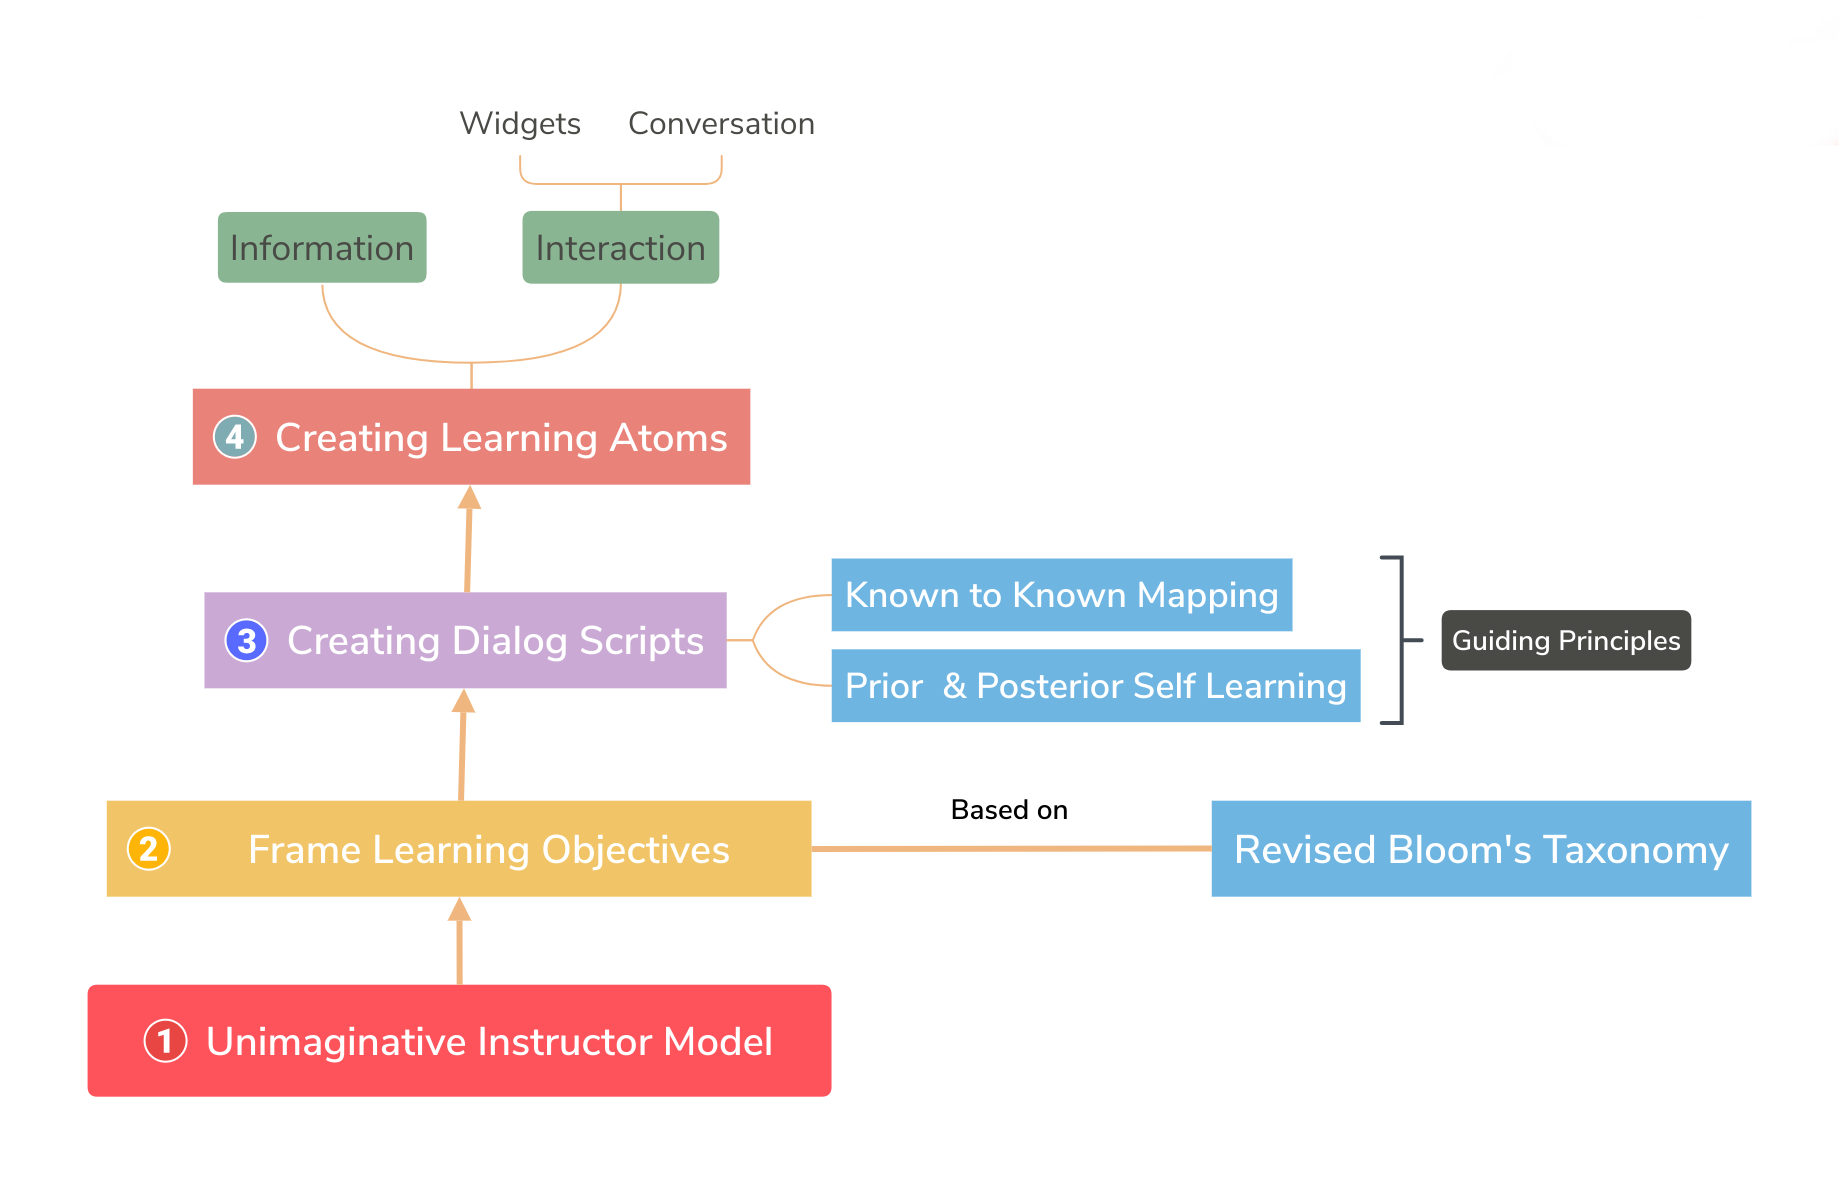
\includegraphics[width=\linewidth]{model.png}
    }
    \caption{The conceptual framework for building course scripts for Primer }
    \label{fig2}
\end{figure}



\subsection[Prior and Posterior]{Principle of Prior and Posterior Self Learning} 


The central idea of conversational learning is to implement Prior and Posterior Learning (PPL). In Prior and Posterior Learning, the agent questions the learner about his prior understanding about a certain topic. After the learner replies his own ideas about the topic, the agent replies with the accepted answer about the topic. The learner can self-evaluate his/her own understanding by comparing against the accepted answer provided by the agent. This lets the user to understand the gaps present in his understanding and accepted understanding in case he is way off. In case the user's understanding of the topic is correct, this reinforces confidence in the learner. 


It can be noted that the agent doesn't offer \textit{correct} answer rather an accepted answer. It is to reinforce the idea that the agent (authority) can be wrong and so can be the accepted answer.  

An example of such Learning Atom is shown is Listing \ref{list4} with the learner Nell who is incorrect in her assumption and an example of such learning where the learner Nell is correct is shown in Listing \ref{list3}.

\begin{lstlisting}[frame=single,caption=Learning Atom with the user having correct assumption ,float,label=list3]
  %*\textbf{Primer}*) : Nell, what do you think is a hypothesis?
  %*\textbf{Nell}*)   : I think a hypothesis is a proposed explanation for a phenomenon. 
  %*\textbf{Nell}*)   : For a hypothesis to be a scientific hypothesis, the scientific         method requires that one can test it.
  %*\textbf{Primer}*) : Simply, hypothesis is an educated guess.
  %*\textbf{Primer}*) : For a hypothesis to be scientific, it has to be a specific,            testable prediction.
  %*\textbf{Primer}*) : It describes in concrete terms what you expect will happen in a        certain circumstance. 
  \end{lstlisting}

  \begin{lstlisting}[frame=single,caption=Learning Atom with the user having incorrect assumption ,float, label=list4]
    %*\textbf{Primer}*) : Nell, what do you think is a hypothesis?
    %*\textbf{Nell}*)   : I think it is an educated guess.
    %*\textbf{Primer}*) : Simply, hypothesis is an educated guess.
    %*\textbf{Primer}*) : For a hypothesis to be scientific, it has to be a specific,            testable prediction.
    %*\textbf{Primer}*) : It describes in concrete terms what you expect will happen in a        certain circumstance. 
    \end{lstlisting}


\subsection[Known-to-Known]{Principle of Known to Known Mapping}


The other principle used to achieve the learning objective of the Learning Atom is named Principle of Known to Known Mapping. It is based on the idea that every topic is built on the foundations of ideas resulting from one or more sets of information. The role of the instructor is often to demonstrate how the topic can be derived from its reference information. Demonstrating such instructing without keeping the learner engaged may result in the learner passively absorbing ideas that may or may not map into the learner's knowledge database. 

\begin{lstlisting}[frame=single,caption=Learning Atom using the principle of Known to Known Mapping,float,label=list5]
  %*\textbf{Primer}*) : Nell, how does the water flow?
  %*\textbf{Nell}*)   : Primer, water flows from higher altitude to lower altitude.
  %*\textbf{Primer}*) : Correct Nell. Now, how does the river Ganges flow in India?
  %*\textbf{Nell}*)   : River Ganga, starts from Himalayas passess through the states          like Uttar Pradesh, Himachal Pradesh, Bihar, West Bengal and then      finally merges with the Bay of Bengal.
  %*\textbf{Primer}*) : If that's the case, what can you comment about the topographical       nature of India.
  %*\textbf{Nell}*)   : The northern parts of India should be at higher elevation and          the slope must gradually lower in the middle part towards the          eastern side of the country.
  \end{lstlisting}
 

In Known-to-Known Mapping, the instructor provides all necessary information as ingredients to derive the required information to the learner and the learner uses the available ingredients to infer the topic's central idea. This is an example of active learning by the learner. This principle is hard to replicate in a live instructor-led classroom due to the constraint of time and in a recorded lecture due to the lack of interactive input. 

A conversational learning agent implements the principle of known-to-known mapping in the following way:
\begin{enumerate}
  
  \item The agent poses questions about the related concept that it believes the learner is aware of
  \item The agent asks the learner to relate the concepts and hints towards the topic objective 
  \item The learner may or may not be able to derive the topic but a sincere effort results in deeper understanding.
  
\end{enumerate}


Such a system ensures that the new knowledge is added to the system maps to something that the learner is aware of and enriches the knowledge database. An example of the principle in action is shown in the Listing \ref{list5}. Here, the learner derives the required information from previously acquired knowledge. The same learning objective is demonstrated using the principle of Unknown-to-Known Mapping in the Listing \ref{list6}. Here, the learner acquires a new piece of knowledge without linking it with exisiting learner's database.  

\begin{lstlisting}[frame=single,caption=Learning Atom using the principle of Unknown to Known Mapping, float,label=list6]
  %*\textbf{Primer}*) : Nell, can you describe the topographical nature of India.
  %*\textbf{Nell}*)   : Nope, Primer. I don't think so.
  %*\textbf{Primer}*) : Well Nell. The northern part of India are at higher altitude and       the altitude tends to decrease as we move towards the southern         part of the country.
  %*\textbf{Nell}*)   : Okay Primer. :|
  \end{lstlisting}


  \begin{figure}
    \makebox[\linewidth]{
      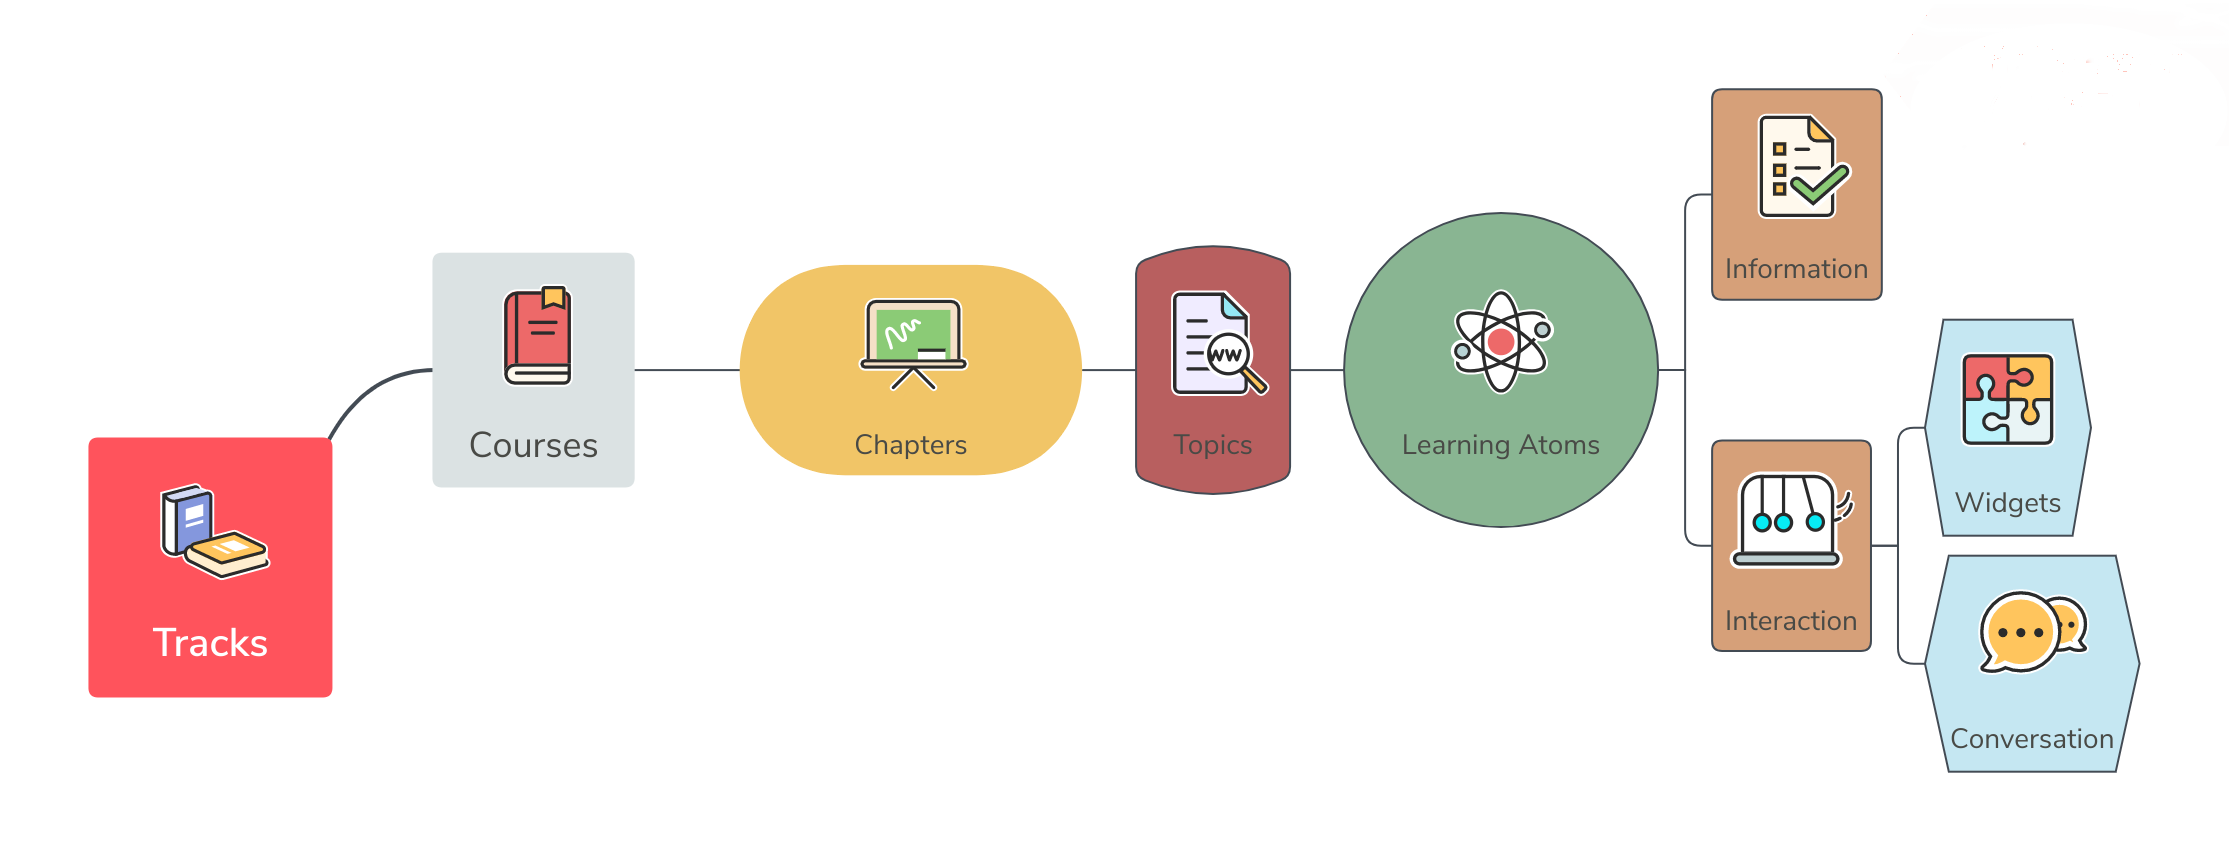
\includegraphics[width=\linewidth]{framework.png}
      }
      \caption{Framework for creation of dialog scripts for Primer }
      \label{fig3}
  \end{figure}

A dialog script is generated based upon the above two principles to achieve the learning objectives of each Learning Atoms. The script is used by the conversational agent to instruct the learner. 



\subsection[Framework]{Framework of Primer Courses}

For creating courses as dialog scripts for Primer, the subject of learning is divided into \textit{Tracks}. An example of Track is \textit{Machine Learning}. Tracks are further divided into courses. For example Machine Learning Track can divided into courses as \textit{Regression, Support Vector Machines etc}. Each course is further divided into \textit{Chapters} and \textit{Chapters} are divided into \textit{Topics}. 

Each Topic is divided into sets of Learning Atoms with a specific learning objective based on Revised Bloom's Taxonomy. Learning Atoms are consist of Information and Interaction. This framework is shown in the figure \ref{fig2} and \ref{fig3}.



This is a basic conceptual framework of the Intelligent Tutoring System, \textit{Primer}. 

Although the tutoring system is ready to instruct the learner, it needs to be extended for a better understanding of the learner. 


\section[Extending the System]{Extending the Tutoring System} 

\subsection[Summarizing]{Summarizing Prompt}
At the end of each topic, the learner is provided with an opportunity to explain their understanding about the recently learned topic. This helps the learners in formulating their understanding of concrete statements in their own language. This learner created summary is also added to an automatically generated notebook at the end of the course.  

If a learner is facing difficulty into explaining the concepts and information, then it is taken into account by the feedback system. How well the dialog script for the topic is able to achieve its learning objective is tracked with Explainability Metric.

\subsection[Explainability]{Explainability and Dialog Script as a Software}

The \textit{Explainability} of the course refers to the fraction of students who took the course and were not able to understand the topic to the total number of learners who completed the course.

This is provided by the students in the feedback system which also asks the students to pinpoint which topic was more difficult to understand too. Feedbacks without reasoning is not taken into consideration for calculating explainability.

Low explainability for a topic demands the course script to modified and improved. This posits the course script to be akin to software which improves itself on every release and is versioned accordingly. The topic which has low explainability can be modified to be divided into smaller parts to facilitate better understanding and the usage of creativity to provide understanding.

In order to deepen the understanding, the course often carries a project component, which the learner needs to complete before the learner can complete the course. 
\begin{figure}
  \begin{equation}
    E = 1 -  \frac{n_s}{n_t}  
  \end{equation}
\begin{align*}
  \text{where}~E &= \text{Explainability of the topic,} \\
  n_s &= \text{number of learners find it lacking to explain the intended topic}\\
  n_t &= \text{total number of learners providing feedback}
\end{align*}
\caption{Calculation of Explainability}
\label{eq:1}
\end{figure}
\subsection[Project]{Project}


The project component of the tutoring system is a tools agnostic dialog script that underlies a real-world problem statement and uses the newly acquired course concepts to solve them. With the help of the project, the agent guides the learner in understanding the application of the topic in the problems. Example of such a project is building a Convolutional Neural Network from scratch and using it for image classification for a real-world dataset.


\subsection[Learner Notes]{Learner Notes}

At any point during the topic or during revision, the learner has the ability to add notes and questions. 

The there system allows different forms of notes:
\begin{enumerate}
  \item \textbf{Topic Notes}: Notes written during the course
  \item \textbf{Revision Notes}: Notes written at the time of revision
  \item \textbf{Questions}: Questions that arise in the mind of the learner
  \item \textbf{Equation Notes}: Notes written against an equation
\end{enumerate}
  
Additionally, all the terms and definition introduced in the topic are compiled together for easier access of the learner. The learner can also coin new terms and its definition for better retention. 

\subsection[Learner Questions]{Learner Questions}

The Tutoring system also includes a community forum where the learner can post their questions. After a certain interval, the questions are compiled and added to the dialog scripts in their next improved version. The tutoring system also helps the learner to document their answer for their questions. 

\subsection[Notebooks]{Automatically Generated Notebooks}


At the successful completion of course, the learner can generate a personalized course notebook in the portable document format(PDF). This document contains lecture notes, learner's notes, learner's responses, terms, and questions.  

This is provided to free the subject of any compulsion during the course to scribble down on paper and provide utmost attention to the topic being taught. The notebook also acts a course journal which can be revisited even after a period of time and will be easier to understand due to its personalized nature.


\subsection[Revision]{Revision and Auto Generation of Flash Cards}
\begin{lstlisting}[frame=none,caption=Automatic Generation of Flash Cards from User Notes,label=list7]
  %*\textbf{User Notes}*) 
    The actual value of the covariance is not meaningful. It's affected by the scale of the two variables. That is why we calculate the correlation coefficient. In order to make something interpretable from the covariance information.

  %*\textbf{Front Side of the Flash Card}*)
    The actual value of the _______ is not meaningful. It's ______ by the ______ of the two variables. That is why we calculate the correlation ________. In order to make something _________ from the covariance information.
  
  %*\textbf{Back Side of the Flash Card}*)
    The actual value of the covariance is not meaningful. It's affected by the scale of the two variables. That is why we calculate the correlation coefficient. In order to make something interpretable from the covariance information.
  \end{lstlisting}

The responsibility of the tutoring system also includes that the learner is able to retain the topics learned during course. After completion of any topic, the learner can revise the topic by going through the conversation with the agent regarding the topic. Also after the topic is completed, predefined flashcards relevant to the topic are added to the revision deck. Apart from that, flash cards are generated from the learner's notes, completed questions and terms. The flashcards generated from user notes is done by first dividing the text into a string of separate sentences and then eliminating the stop words from the sentence. Stop words are the words in the language which appear frequently but doesn't provide additional meaning to the sentence. An example of the autogenerated flash card from the user notes can be seen in the Listing \ref{list7}.

\subsection[Retention]{Retention}

The responsibility of the agent includes ensuring that the subject retains the course in the long term. In order to do that, there are two kinds of facilities for revision provided:
\begin{itemize}
  \item \textbf{Spontaneous Revision of Topic}: 
  After the completion of any topic, the spontaneous revision option is enabled and the subject can go back and browse through the conversations with the agent. Completing the flashcards associated with the topics is considered as the completion of revision.
  \item \textbf{Scheduled Revision of Topic}: 
  Once the course is completed,  in order to ensure that the effort spent during learning the course is not wasted, the conversational agent draws up a revision schedule. 
  
\end{itemize}


The revision schedule consists of a five-term revision separated at certain intervals of days in order to implement Spaced Repetition. The revision schedule is based on mean average \textbf{retention score} for all the topics present in the course. 


\subsection[Retention Score]{Retention Score}


Retention score is calculated for each topic with the following equation:

\begin{figure}[!ht]
  \begin{equation}
    R = 10e^{\frac{-t}{s}}
  \end{equation}
\begin{align*}
  \text{where}~R &= \text{Retention Score,} \\
  t &= \text{time passed since topic or revision session completion} \\
  s &= \text{Retention Strength of the topic}
\end{align*}
\caption{Retention Score Calculation}
\label{eq:2}
\end{figure}


Retention Strength has a base strength. It is increased when scheduled revision is performed and also when the learner's notes are modified regarding the topic.
Retention Strength depends on:
\begin{itemize}
  \item Number of topic notes the user has added
  \item Number of revision notes the user has added
  \item Number of questions the user has proposed and answered
  \item Number of terms the user has defined
  \item Number of Equation Notes the user has defined.
\end{itemize}
  
Retention score has been created to put a quantitative figure on the subject's retention. Though there is no evidence for any correlation existing between the retention score and the actual retention, it acts as a proxy for putting a number to the decaying knowledge. 
\begin{itemize}
  \item When the user completes the topic, R = 10 with t = 0. As time passes the Retention score decreases while strength remains constant.
  \item When a person completes a scheduled revision, revision is reset to 10 and strength goes up. Though spontaneous revision resets the retention score to 10, it doesn't affect the retention strength. 
\end{itemize}

The purpose of Strength is to add an incentive whose effect is visible to the user. The following figure demonstrates the visible effects of revision.


\begin{figure}[!ht]
  \makebox[\linewidth]{
    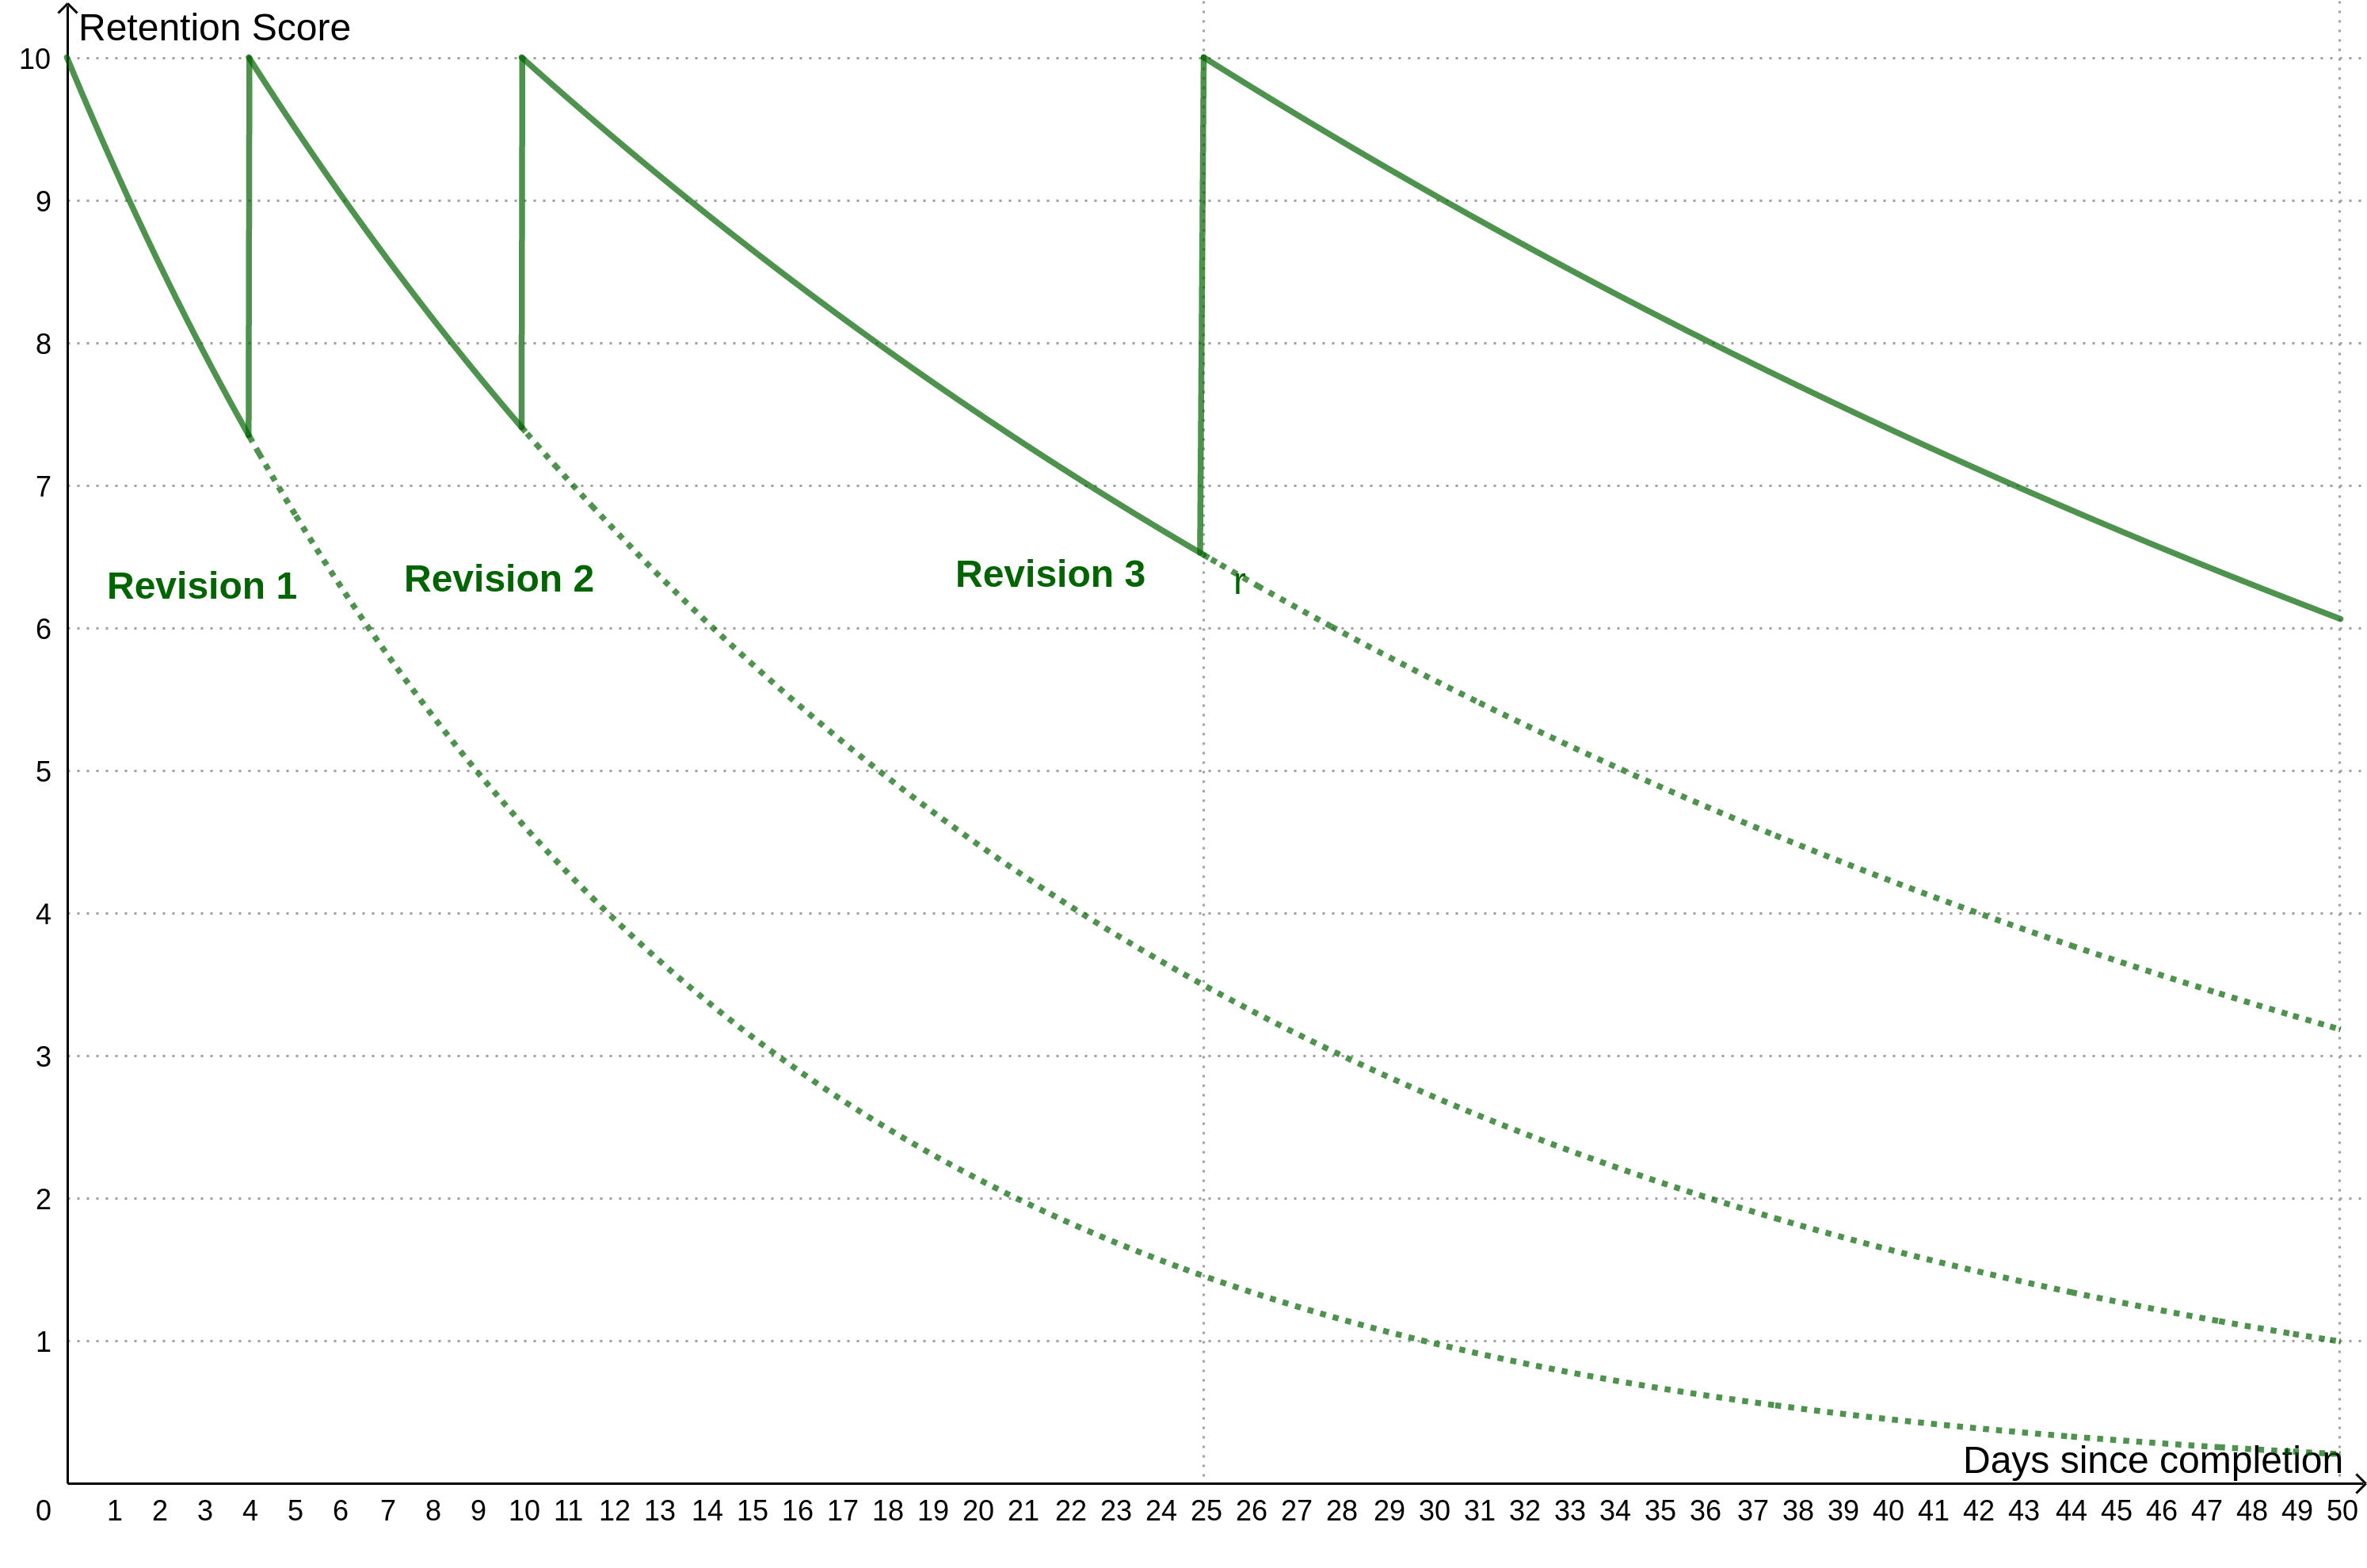
\includegraphics[width=1\linewidth]{sr4.png}
    }
    \caption{Retention Score plot against time passed since completion in days. Revision shown here are scheduled revision.}
    \label{fig6}
\end{figure}


\subsection[Incentives]{Incentives for completing the course and revision}

The tutoring system takes into account that the learner will lack the discipline to complete through the course or to revise the contents frequently. In order to deal with the issue, the system incorporates incentives.
\begin{enumerate}
  \item Incentives for course completion is that the personalized notebook and flash cards are generated only after course completion.
  \item Incentives for revision is to keep up the retention score  
  \item Incentives for adding notes, terms, and questions is to increase the retention strength for the retention score.
\end{enumerate}



The intelligent tutoring system outlined above is a basic framework for building a dialog based tutoring system. It has been designed to be extensible, customized to the needs of the topic. Such a system will help anyone who wishes to learn difficult topics without a human actor.


\section[Advantages]{Advantages of the tutoring system}
The tutoring system is an effective tool as a standalone software as well as an aid to the educators.
\begin{enumerate}
  \item \textbf{Extensible System }: The features of the tutoring system can be extended to accomodate features that help the learner learn.  
  \item \textbf{Faster completion}: Text based interactive courses on average takes less than 50\% of the time to complete than video based courses.   
  \item \textbf{Persistent Attention Span}: The text based interactive courses help the learner to have greater attention span as the tutor doesn't proceed without the input of the learner.     
  \item \textbf{Complete Learning Framework}: The intelligent tutoring system helps learners learn, understand and retain. 
  \item \textbf{Journaling}: The interactions and conversations with the system serves for journaling purpose. 
  \item \textbf{Identifation of Knowledge Gaps}: The system allows the assessment of the learner's understanding at a low level using Learning Atom. This allows for learners to self evaluate the gaps they have in their knowledge and self-correct.
  \item \textbf{Fast Iteration of Courses}: The course scripts can be improved upon feedback for the learners. As opposed to video based courses, the text based courses can be iterated rapidly.   
\end{enumerate}


\section[Limitations]{Limitations of the system}
\begin{enumerate}
  \item \textbf{Tacit Knowledge}: Although, the framework can be used to convey explicit knowledge, tacit knowledge can be difficult to convey through the medium. It refers to the kind of knowledge that is difficult to transfer to another person by means of writing it down or verbalizing it. Examples can be learning to ride a bike etc. 
  \item \textbf{Cannot replace human}: A personalised dialog based assistant cannot match the effectiveness of an efficient human tutor. However, it can set it as a benchmark and can be improved to move towards that direction.
\end{enumerate}


\section{Future Scope}
\begin{itemize}
\item \textbf{Addition of Natural Language Processing Abilities} The blueprint of the tutoring system demonstrated above shows that a dialog based agent doesn't require the abilities to process natural language. However, incremental addition of such capabilities can be added to better facilitate learning and being more adaptive to the learner's need.
\item \textbf{Building a social simulation game} Some tacit knowledge are learnt when the learner interacts with the real world. This cannot be communicated directly to the learner. A social simulation game which is sub-genre of the Life Simulation game can be an effective platform to learn such knowledge. Examples of such game include The Sims Series by EA, Animal Crossing etc. The game can be modified to mimic the real world with programming of actions and their resulting consequences. This game can be used by the tutoring system, Primer to boot up relevant scenario for the learner and acting as a guide in the game. For example, if the learner wishes to learn what does it take to become a politician, a game with the setting for the protagonist to be a politician can be booted up. This will enable the learner to learn through exploration and virtual experience.   
\end{itemize}

\section{Conclusion}
We have proposed a tutoring system using a dialog based agent without the agent possessing capabilities of processing natural language. We started with the usual framework of an instructor model and converted it into scripts which can be used by the conversational agent to instruct learner. This was done by using Revised Bloom's Taxonomy to frame learning objectives and using principles of Known-to-Known Mapping and the Prior and Posterior Self-Learning. The system was extended using features such as automatic notebook generation, automatic flash cards generation and spaced repitition to enable the learner retain the course concepts for a longer time. Though, the system might be ineffective at the beginning, it can be improved by additions of new features and iterations of course scripts based on the Explainability metric. 

\section{Acknowledgements}
The project had its genesis in Early 2014, when Mr.Pawan Gupta of Society of Integrated Development gave a lecture at the author's university on the ancient education system of India.\cite{gupta2000liberating} The example shown in Listing \ref{list4} and inspiration for the Principle of Known-to-Known Mapping is taken from that lecture. 

We also thank author Neal Stephenson whose work, The Diamond Age \cite{stephenson1998diamond}, captivated the author's mind of the possibilities that a teaching machine can possess.

We would also like to show our gratitude to Mr.Pawan Mohata, Workloop Co-working Space, Bhubaneswar for letting the author work at his co-working space and deferring the payment of the rent till the project makes any money. Without his invaluable support, this project might have never been completed.
\section{Exhibits}

\addtocontents{toc}{\protect\endgroup}
\medskip
\addcontentsline{toc}{section}{References}
\bibliography{article}
 \thispagestyle{plainx}
\end{document}
